\documentclass[12pt]{article}

\usepackage[]{amsmath}
\usepackage[]{amsthm}
\usepackage[]{amsfonts}
\usepackage[]{amssymb}
\usepackage{blindtext}
\usepackage[a4paper, total={7.5in, 10in}]{geometry}
\usepackage{graphicx}
\usepackage{listings}
\usepackage{color}
\usepackage{array}
\usepackage{wrapfig}
\usepackage{hyperref}
\usepackage{float}

\definecolor{dkgreen}{rgb}{0,0.6,0}
\definecolor{gray}{rgb}{0.5,0.5,0.5}
\definecolor{mauve}{rgb}{0.58,0,0.82}

\pagenumbering{arabic}
\let\cleardoublepage\clearpage


%% parameters for code snippets, etc (to put a keywords and smaller snippets inline, use \texttt{} tag
\lstset{frame=tb,
  language=Java,
  aboveskip=3mm,
  belowskip=3mm,
  showstringspaces=false,
  columns=flexible,
  basicstyle={\small\ttfamily},
  numbers=left,
  numberstyle=\small\color{black},
  keywordstyle=\color{blue},
  commentstyle=\color{dkgreen},
  stringstyle=\color{mauve},
  breaklines=true,
  breakatwhitespace=true,
  tabsize=4
}

%%title of document
\title{Concrete Architecture Analysis of OpenPilot}



%%ADD NAME AND STUDENT NUMBER HERE
\author{
    \textbf{Jerry Wu} (jerrywu0@my.yorku.ca), \textbf{Joseph Spagnuolo} (joe13@my.yorku.ca),\\ \textbf{Tarun Bhardwaj} (tarunb4@my.yorku.ca),
    \textbf{Krishna Raju} (krishnar@my.yorku.ca),\\ \textbf{Irsa Nasir} (inasi022@my.yorku.ca),
    \textbf{Aish Singh} (aish19@my.yorku.ca),\\ \textbf{Stanley Ihesiulo} (ihesiulo@my.yorku.ca),\\
    \textbf{Connor-Francis McGrath} (connorm3@my.yorku.ca)
}



%%due date
\date{Due Mar 10 2024}

\begin{document}
\maketitle
\tableofcontents

\newpage
\section*{Abstract}
This paper is a follow up to our last paper on the conceptual architecture of openpilot by comma.ai. It will go over the concrete architecture of the system as a whole, as well as the architecture of one specific subsystem: \texttt{localization/calibration}. This information was extracted from the project's source code (version 0.9.5) using the Understand software by scitools. Our findings indicated that, after extracting the concrete architecture of the system, that openpilot uses a \textbf{layered architecture} for the whole system in general, as well as a \textbf{pipe and filter} architecture. This is a direct correlation to our findings during our conceptual architecture analysis of the system in the previous paper.

\section{Introduction and Overview}
Previously, the group discussed the conceptual architecture of the openpilot advanced driver assistance system developed by comma.ai. The architectural models the group discussed were derived from documentation provided both by comma.ai as well as external sources. Now, the group has spent time analyzing the concrete architecture of openpilot. By exploring the structure of the file directories, file dependencies, as well as analyzing source code in the Understand software, the group came to understand the concrete architecture of the software, which will be explored in this report.

Firstly, the concrete architecture of the entire software system will be analyzed using Understand to become aware of folder structure and dependencies among the files. By scrutinizing the Understand graphs, the group came to the conclusion that the layered architecture style suits the overall openpilot system the closest. This is a similar conclusion the group came to in the conceptual analysis. However, looking at the file structure in Understand highlighted how the conceptual architecture the group created did not fully capture all nuances and dependencies that actually occurred in the openpilot software, which will be discussed later in the architecture section of this report.

In addition to browsing the overall file architecture of openpilot, the group also went into detail analyzing the localization and calibration subsystem. From there, the group concluded that a pipe and filter architectural style best suited the localization subsystem, due to how the files in the localizationd folder get input from an input data stream, calculate the required values, resulting in an output that acts as the input for a separate file to determine localization properties of the vehicle. When it came to the calibration system, the group found that while no architectural system seems to fit directly, the pipe and filter architecture is the closest fit that captures the functionality of the calibration system.

Not only will the architectures be shown, but the derivation process as well, so that others reading will be able to understand and duplicate the method undertaken to derive the architectural styles of openpilot. In general, the derivation process consisted of: downloading openpilot version 0.9.5 from comma.ai's github, opening the project folder with Understand, analyzing the file architecture graph of the entire system, from there finding a particular subsystem and analyzing the file architecture and dependencies in order to find out how subsystems interact with one another.

\section{Concrete Architecture of Openpilot}

\subsection{File Architecture of Openpilot}

In order to find out the architecture of openpilot, it is necessary to look at the file architecture and dependencies within Understand.

    \begin{figure}[H]
        \centering
        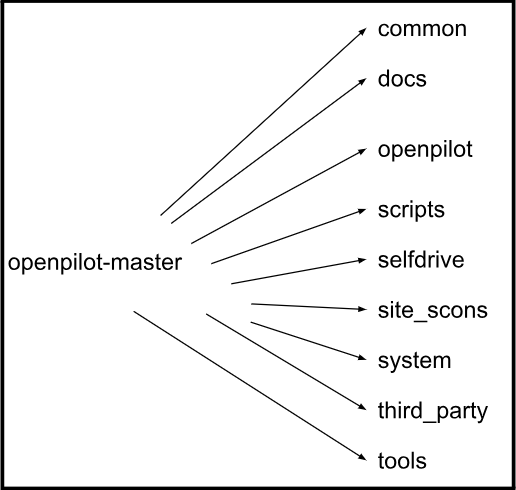
\includegraphics[scale=0.75]{openpilot architecture.png}\\
        \caption{A recreation of the Understand graph detailing the subfolders within the openpilot project}
        \label{fig:enter-label}
    \end{figure}

After dissecting the architecture of the overall software system, the group figured out that the main subsystems that made up openpilot's functionalities were: common, third\textunderscore party, tools, system, and selfdrive.
\vspace{10pt}

Their individual functions include:
\begin{itemize}
    \item common - A common place where many of the subsystems call upon its functionalities. We can see in the dependency diagram for common, selfdrive, system, and tools all depend on functions within common.
    \item third\textunderscore party - External third party tools such as JSON and Kaitai parsing tools.
    \item tools - Contains shell scripts for setting up openpilot on different operating systems. As well as functionalities for running the comma device and other peripheries.
    \item system - Provides many services for setting up system attributes such as: reading audio measurements, setting the time and timezone, publishing log messages. Also contains subfolders that perform important driving functionality including:
        \begin{itemize}
            \item Camerad – Captures video [5]
	    \item Loggerd – Records driving and analyzes data [5]
	    \item Sensord – Sensor reading [5]
	    \item Ubloxd – Handles GNSS data (parses for location services) [5]
        \end{itemize}
    \item selfdrive - Handles self driving functionality, such as transforming the video with the neural network, provide localization based on data from the System subfolder, and facilitate communication between the panda and the software. Also contains subfolders that perform important driving functionality including:
        \begin{itemize}
            \item Locationd – Provide localization (using data from ubloxd) [5]
	    \item Boardd – Communication between panda and openpilot                  software. Acts as publisher for messages [5]
	      \item Modeld – Transforms the video with the neural network [5]
	      \item Thermald – Monitor thermal state of the device running openpilot. Additionally, monitors other properties such as CPU and RAM usage, as well as power status [5]

        \end{itemize}
\end{itemize}

\subsection{Architectural Style of Openpilot}

    The group came to the conclusion that the architectural style that best suited the entire openpilot system is a \textbf{layered} architectural style. This conclusion was reached after looking at dependency diagrams in Understand.


    \begin{figure}[H]
        \centering
        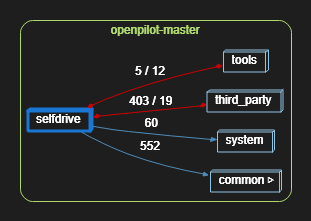
\includegraphics[scale=1]{Dependencies-selfdrive.png}\\
        \caption{selfdrive's dependency graph from Understand. Here it is apparent that there are two way dependencies between selfdrive and third\textunderscore party, as well as a one way dependency towards common}
        \label{fig:enter-label}
    \end{figure}

    \begin{figure}[H]
        \centering
        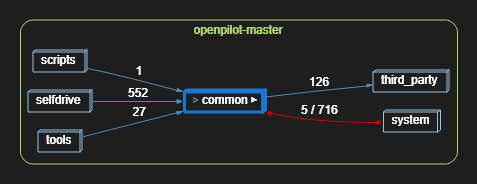
\includegraphics[scale=1]{Dependencies-common.png}\\
        \caption{common's dependency graph from Understand. There is a one way dependency between common and third\textunderscore party.}
        \label{fig:enter-label}
    \end{figure}

    \begin{figure}[H]
        \centering
        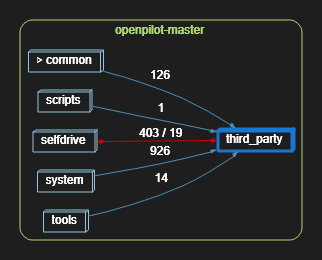
\includegraphics[scale=1]{Dependencies-third_party.png}\\
        \caption{third\textunderscore party's dependency graph from Understand. Here the dependencies between common and selfdrive}
        \label{fig:enter-label}
    \end{figure}

    \begin{figure}[H]
        \centering
        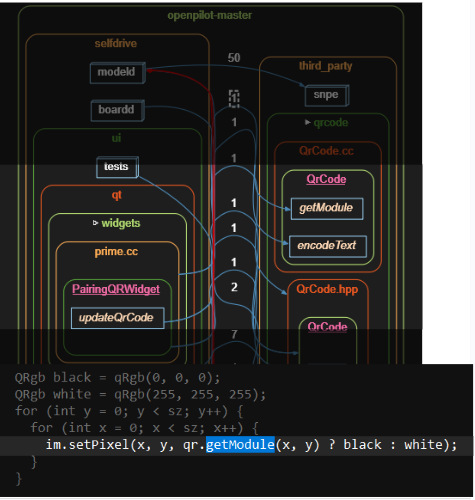
\includegraphics[scale=1]{getmodule.png}\\
        \caption{One of the dependencies between selfdrive and third\textunderscore party. Within selfdrive, the updateQrCode calls on the getModule method within third\textunderscore party}
        \label{fig:enter-label}
    \end{figure}

Within Figure 2, 3, and 4, as well as the file architecture of the whole system, there is clear segmentation between subsystems based on functional purpose. Additionally, looking at the dependencies, certain subfolders, such as selfdrive have dependencies on folders such as common and third\textunderscore party. From here it is possible to model selfdrive as a higher layer than third\textunderscore party with common as an abstraction layer in between. However, as seen with selfdrive's direct dependency on third\textunderscore party, the system allows for non-adjacent communication, as seen in Figure 5.

It is important to note, that the layered architecture the group came up for the conceptual design does not match the concrete architecture seen in the Understand file. It is an important lesson that conceptual models of software often do not capture the complexities and nuances of an actual software architecture, and while they remain important frames of reference, it is often the case that the needs of the software, whether they be for performance or any other reason, will stray away from these architectural models.

In this case, although it was stated that selfdrive was a higher layer separated from third\textunderscore party by common, there is still two way communication between the two that is non adjacent, meaning the previous conceptual model did not capture that relationship, and should be changed to accommodate it.

\subsection{Design Patterns}
\begin{itemize}
    \item[1.] Creational Pattern:
        \begin{itemize}
            \item \textbf{Singleton}:
            OpenPilot might use Singleton for managing access to critical system resources or services, such as the manager for all subprocesses or the configuration manager, ensuring that only one instance is created and accessible throughout the system.
        \end{itemize}

    \item[2.] Structural Pattern:
        \begin{itemize}
            \item \textbf{Adapter}:
            OpenPilot interfaces with a variety of hardware and sensors. The Adapter pattern could be used to standardize the interface between the software and different hardware components, such as cameras, radars, and GNSS modules, allowing them to communicate seamlessly despite potential differences in their interfaces.
        \end{itemize}

     \item[3.] Behavioral Pattern:
        \begin{itemize}
            \item \textbf{Observer}:
            In OpenPilot, the Observer pattern could be used for handling sensor data updates, where the sensor data processing subsystem acts as the subject, and various components of the system (like neural network runners or the localization system) act as observers, updating their state based on the sensor data.
        \end{itemize}

\end{itemize}

\subsection{Description of Top-Level Subsystems and Interactions}

Within the OpenPilot software there are five major subsystems that comprise the system to ensure the software is functioning correctly. 

\begin{itemize}
    \item[1.] Sensors and Actuators:
        \begin{itemize}
            \item \textbf{boardd}: which manages communication between the panda and the openpilot software. It enables the transmission of control commands to the car and receives data from car sensors [1].
            \item \textbf{camerad}: which processes image data from the car’s cameras. These images are crucial for the neural network to make driving decisions and monitor the driver's attention [1].
            \item \textbf{sensord}: which handles IMU and additional sensor data reading from gyroscopes, accelerometers, and light sensors. Providing essential information about the car's movement and environment [1]. 
        \end{itemize}
    \item[2. ] Neural Network Runners:
         \begin{itemize}
            \item \textbf{modeld}: Uses the image stream from the cameras processed by camerad and inputs from the sensors managed by boardd and sensord, running the driving neural network to determine the driving path and make decisions [1].
            \item \textbf{dmonitoringmodeld and dmonitoringd}: Utilize the driver-facing camera stream to ensure the driver is attentive and capable of taking control if necessary [1].
        \end{itemize}
    \item[3. ] Localization/Calibration:
        \begin{itemize}
            \item \textbf{ubloxd}: Parses GNSS data for localization [1].
            \item \textbf{locationd}: Which uses a Kalman filter service to provide precise vehicle localization [1].
            \item \textbf{calibrationd}: Calibrates the camera to align it with the vehicle’s frame [1].
            \item \textbf{paramsd}: Which adjusts the vehicle parameters for more accurate control [1].
            \item This information is critical for the neural network runners to make informed decisions.
        \end{itemize}
    \item[4. ] Controls:
        \begin{itemize}
            \item \textbf{radard}: Processes radar data for detecting objects and tracking them [1].
            \item \textbf{plannerd}: Laterally and longitudinally calculates the path planning [1].
            \item \textbf{controlsd}: Generates and sends the control commands to the actuators of the vehicle [1].
        \end{itemize}
    \item[5. ] System, Logging, and Miscellaneous Services:
        \begin{itemize}
            \item Services like \textbf{manager}, \textbf{thermald}, \textbf{loggerd/logcatd/proclogd, athenad}, and \textbf{ui} support the core functions by managing service lifecycles, monitoring device health, handling logs for analysis and improvement, connecting to remote services for updates and assistance, and providing the user interface [1].
        \end{itemize}
\end{itemize}
The interaction flow within OpenPilot follows a structured and efficient pathway. Starting with the data collection, where sensors and cameras diligently gather comprehensive environmental and vehicular data. Next, this gathered data then serves as the foundation for the next phase which is data processing. Here data feeds into the neural networks (modeld, dmonitoringmodeld) for processing. Localization and calibration plays an important role to ensure that the vehicle's exact position and orientation are accurately determined.  Once the neural networks have analyzed the data and made their decisions, it is then passed to the controls subsystem, which is tasked with translating these decisions into tangible vehicle controls, adjusting the vehicle's path and speed as necessary to adhere to the planned route. Supporting this entire process, the system, logging, and miscellaneous services provide essential infrastructure support, covering aspects such as device monitoring, data logging for future enhancements, and user interface management [1].




    


\subsection{Architecutral Style of Localization/Calibration}
While we discovered that the system as a whole follows a layered architectural style, delving deeper into the Localization, as well as the Calibration modules, we found out that these share a different architecture than the system as a whole. From our investigation, it seems to be that both the Localization and the Calibration modules makes use of the pipe-and-filter architectural style.


To extract the concrete architecture of the Localization module, we used the dependency diagram generated by the “Understand” program, from the source code. The figure below shows the dependency diagram from which the concrete architecture of the Localization module was derived. As can be seen in the diagram, when we focus on the dependencies of the localization module and the functionality of each sub-module within it, we see that it largely consists of modules which are responsible for gathering data from outside sources, and modules which are responsible for processing that data. 


\begin{figure}[H]
    \centering
    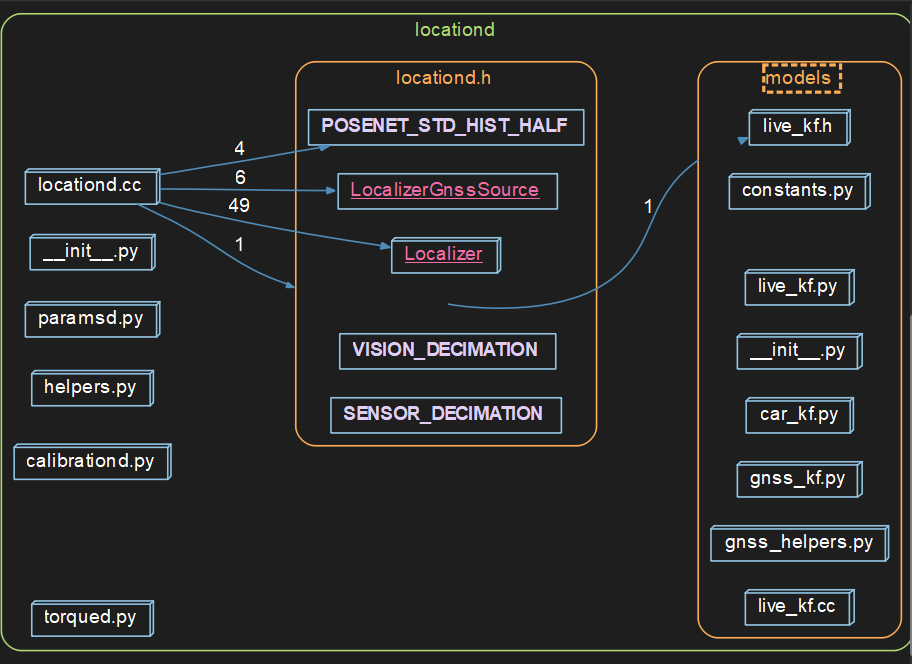
\includegraphics[scale=0.4]{extracted-architecture-understand.png}\\
    \caption{Extracted architecture of the "Localization" subsystem from Understand}
    \label{fig:enter-label}
\end{figure}

As seen in the image, the LocalizerGnssSource module is responsible for collecting data from the system sensors and controls to be used to localize the vehicle. Then, in a pipe-and-filter manner, this data is then passed on to the 'models' submodule, responsible for using this data to predict the localization properties of the vehicle, such as the wheel odometry and other localization features. The "torqued" submodule is also used for this same predictive purpose - for predicting the torque of the vehicle. The other modules within the localization subsystem are mostly just constant definitions, and calibrating the predictors to the specific vehicle.

From this architecture extracted from Understand, we grouped the architecture of the Localization submodule into four modules which follow a pipe-and-filter architecture:
\begin{itemize}
    \item[1.] Calibration
    \item[2.] Localization sources
    \item[3.] Predictors
    \item[4.] Messaging
\end{itemize}

This pipe-and-filter architecture is illustrated in the figure below showing the concrete architecture of the Localization subsystem: The calibration submodule first calibrates the predictors to the specific features of the vehicle; The "Localization Sources" submodule is responsible for the gathering of sensor and control data for the purpose of vehicle localization; The "Predictors" submodule is reponsible for taking this localization data from the localization sources subsystem and using it to predict vehicle localization properties; and finally, the output of the "Predictor" subsystem is passed on to the rest of the system through the "celery" messaging system which will be discussed more in detail later. This is a straightforward application of the pipe-and-filter architectural style, where data sources are received, passed on, and processed.
\begin{figure}[H]
    \centering
    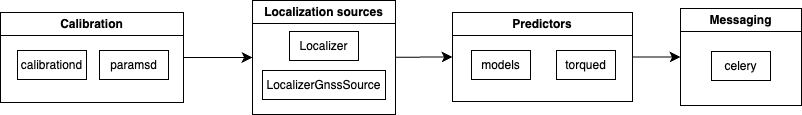
\includegraphics[scale=0.5]{concrete-architecture-localization.png}\\
    \caption{Concrete architecture of the Localization subsystem}
    \label{fig:enter-label}
\end{figure}

The Calibration subsystem, as the name implies, is responsible for calibrating the predictors to the specific vehicle being used. This subsystem follows much the same architecture as the Localization subsystem: it uses the pipe-and-filter architecture.

We followed the same process of extracting an architecture from understand of the calibration subsystem. This, however, did not give us much to go off of, as this subsystem has a mostly flat directory structure, and does not have much structure in terms of its program hierarchy. Most of what can be found are definition of constants which are used in the subsystem, as well as modules which have no dependency, responsible for implementing the algorithms required for calibration (such as the `moving\_average\_with\_linear\_decay` module). 

\begin{figure}[H]
    \centering
    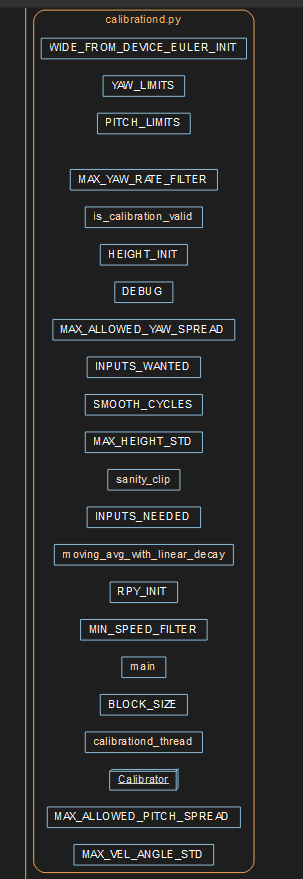
\includegraphics[scale=0.5]{extracted-architecture-calibration.png}\\
    \caption{Extracted architecture of the Calibration subsystem}
    \label{fig:enter-label}
\end{figure}

Given the simplicity of this subsystem, we concluded with the pipe-and-filter architecture outlined in the image below, the first module being the "Constants" module, where required constants are defined, then the "Calibration algorithms" module, which implement algorithms required for calibration, and finally the "Messaging" module, which outputs any relevant calibration information to the rest of the system. 

\begin{figure}[H]
    \centering
    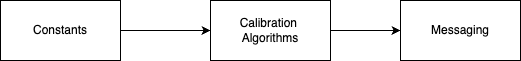
\includegraphics[scale=0.5]{concrete-architecture-calibration.png}\\
    \caption{Concrete architecture of the Calibration subsystem}
    \label{fig:enter-label}
\end{figure}

\subsection{Derivation Process of OpenPilot Architecture and Localization/Calibration Architecture}

The following are the steps that we took to derive the concrete architecture of the system as a whole, as well as specifically how to access the architecture for locationd:

\begin{itemize}
    \item[1.] Firstly, we went on the Understand software's website and received a license key via email
    \item[2.] We then opened the root folder for the openpilot project on version 0.9.5
    \item[3.] We made sure to ignore the program's prompt to compile the code, as the project was large and compilation wouldn't be necessary to perform static code analysis
    \begin{figure}[H]
        \centering
        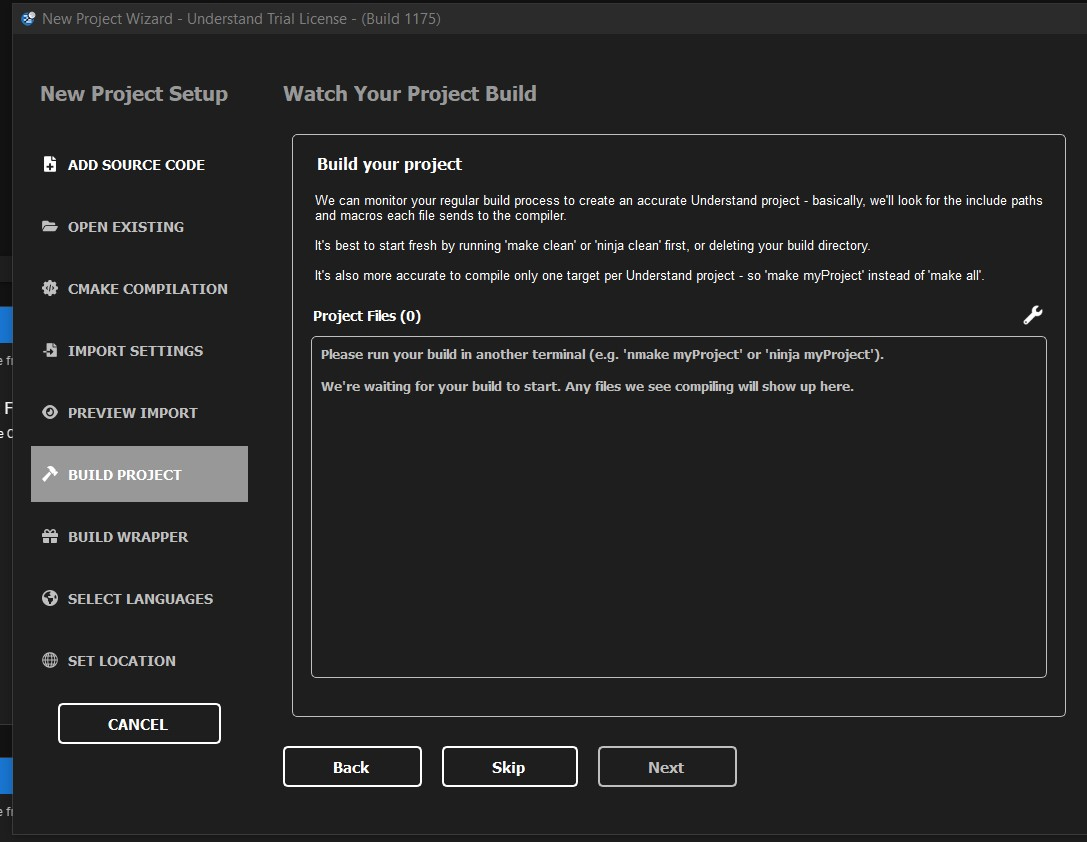
\includegraphics[scale=0.3]{importing.jpg}\\
        \caption{The window which shows up when importing a new project into Understand}
        \label{fig:enter-label}
    \end{figure}
    
    \item[4.] Once the project has been opened in Understand, we looked through the project at the file level and had access to architecture and dependency diagrams that were automatically generated by the software
    \item[5.] To access \texttt{locationd}, we went into the project browser (the top left panel as illustrated) and found \texttt{locationd.h}

    \begin{figure}[H]
        \centering
        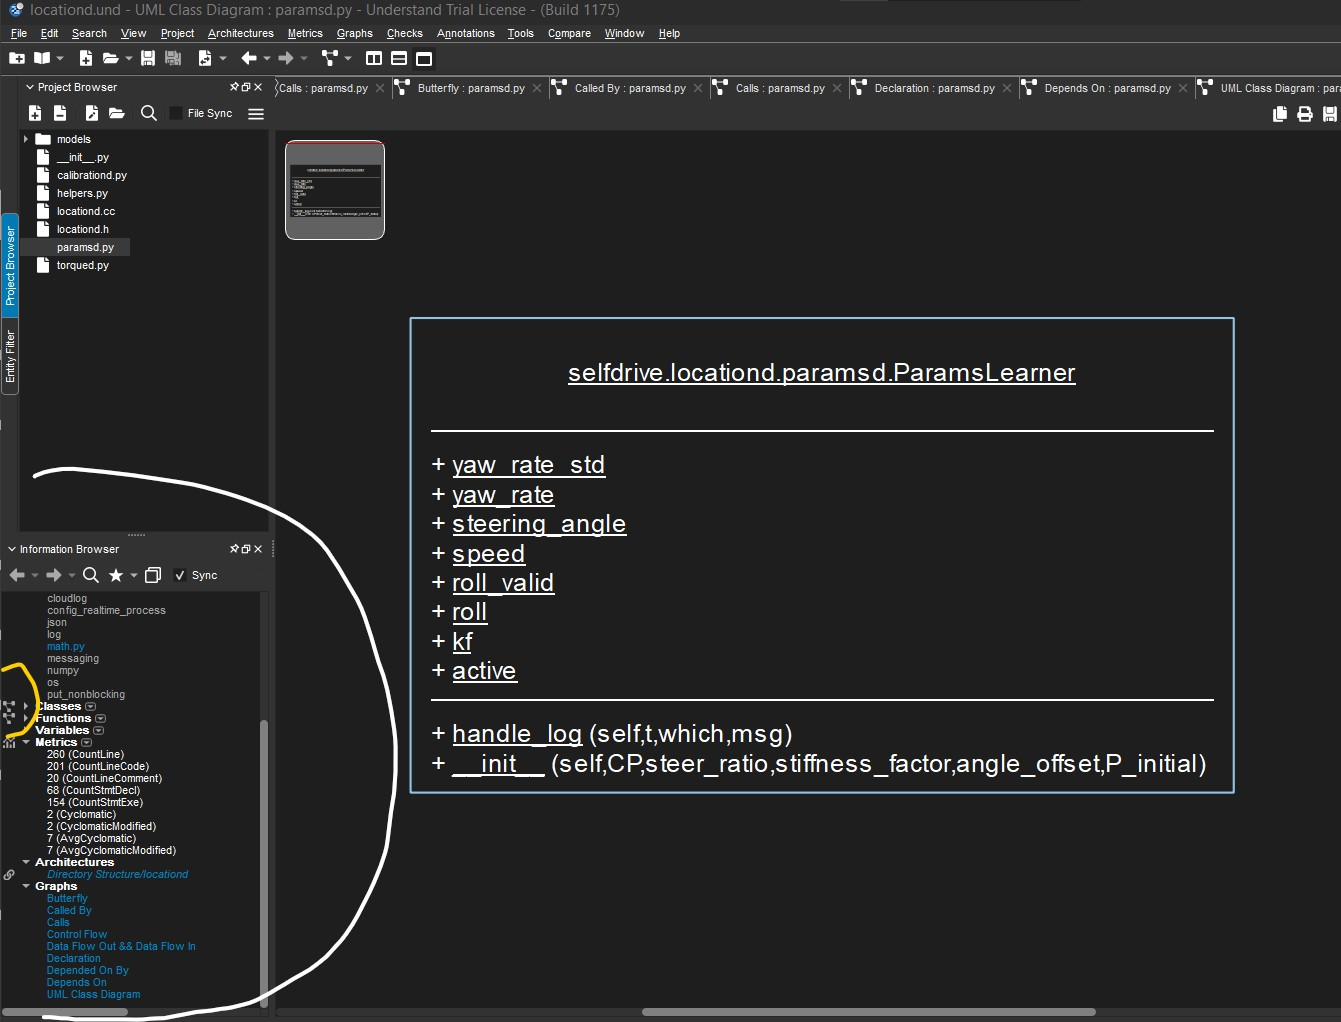
\includegraphics[scale=0.2]{understand.jpg}\\
        \caption{The white circle indicates the information browser and the yellow circle is the icon}
        \label{fig:enter-label}
    \end{figure}

    %%ADD SCREENSHOTS OF UNDERSTAND

    \item[6.] Finally, we go into the panel under project browser labelled "information browser" and clicked on the small icon with three dots in a triangular arrangement to view the architecture diagram for \texttt{locationd}
\end{itemize}

\subsection{Concurrency In The Localization/Calibration Subsystem}
Concurrency is present in the localization/calibration subsystem and is enabled using the Cereal messaging framework. Cereal allows components to broadcast data streams that other components can subscribe to facilitating real-time, asynchronous exchanges between subsystems via a publish-subscribe model.
    
\begin{itemize}
    \item \textbf{locationd} fuses data from GPS, cameras, and IMUs to accurately determine the car's position, using Kalman filters for precision.
    \item \texttt{calibrationd} continuously adjusts the camera feed to account for lens distortion and misalignment, ensuring that the system receives a consistently clear and accurate visual input.
    \item \texttt{ubloxd} processes GNSS data in real-time, enhancing the vehicle's location accuracy by working with other localization subsystems.
    \item \texttt{paramsd} dynamically updates OpenPilot's parameters based on sensor inputs, optimizing the system's responses to real-time driving conditions.
\end{itemize}

\subsection{Team Issues in Localization/Calibration subsystem}
The following are 2 development issues that were present in the localization/calibration subsystem:

\begin{itemize}
    \item \href{https://github.com/commaai/openpilot/pull/26460}{\#26460 "[locationd] Add input checks”} : In the location subsystem, unreliable data from sensors was leading to degradation in the localization subsystem’s performance. The issue was fixed by adding enhanced input validation in locationd to identify and disregard unreliable data before it could adversely affect the localization process. 
    \item \href{https://github.com/commaai/openpilot/issues/21303}{\#23284 “paramsd: bad init while in a turn”} : In the paramsd subsystem, inaccurate parameter values were being estimated due to a delay in camera0demetry messages during device initialization during turns. This inaccuracy impacted the system's decision-making processes and response during turns. The issue was fixed by adding a check if all messages are valid before starting the filter.
\end{itemize}

\section{Diagrams}

\subsection{Use case}

Below is a use case diagram illustrating the main actor (the driver) making a request for navigation assistance while using openpilot. The \texttt{locationd} module will receive data from the GPS, whereby it will process the data and send the location data back to the user via the software's user interface.

\begin{figure}[H]
    \centering
    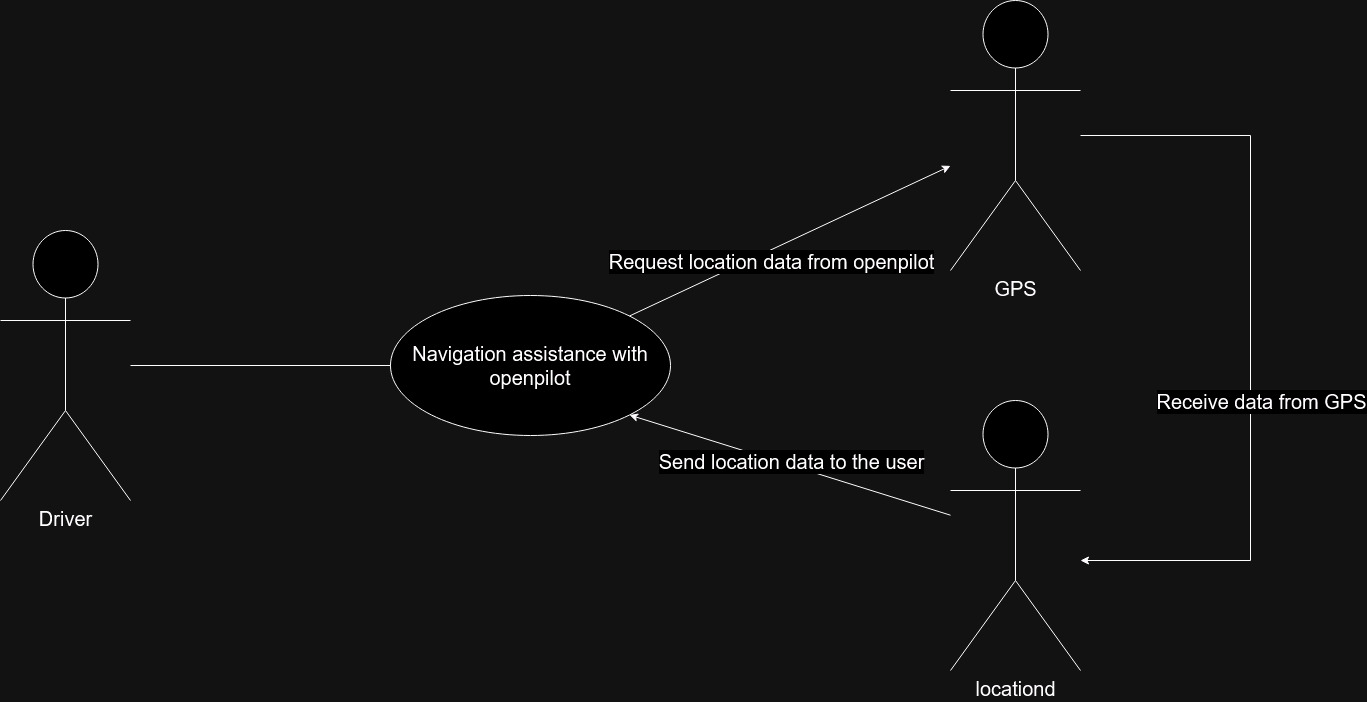
\includegraphics[scale=0.2]{usecase.jpg}\\
    \caption{Navigation assistance use case for \texttt{locationd}}
    \label{fig:enter-label}
\end{figure}

\subsection{Sequence diagrams}
The following sequence diagrams illustrate the core functionalities of \texttt{locationd} and \texttt{ubloxd}. 
In the \texttt{ubloxd} system first \texttt{ubloxd} creates an instance of \texttt{PubMaster} which handles publishers and subscribers, The \texttt{PubMaster} then creates a socket connection to the \texttt{ubloxGNSS} module. Then \texttt{ubloxd} creates a \texttt{ubloxmsg} and populates it with data then it sends it to the \texttt{PubMaster} which sends it to \texttt{ubloxGNSS}. This process is repeated in a loop constantly supplying \texttt{ubloxGNSS} with updated Ublox data.

In the \texttt{locationd} system, \texttt{locationd} first creates a \texttt{Localizer} object which gets the availability of the Ublox system from \texttt{paramsd}. the \texttt{Localizer} subscribers to gps location data from \texttt{ubloxGNSS} via the \texttt{SubMaster}. Then \texttt{ubloxGNSS} publishes data to \texttt{SubMaster} which then forwards it to \texttt{Localizer}  who is a subscriber \texttt{Localizer} then returns the data to \texttt{locationd} and the process repeats providing updated location data from \texttt{ubloxGNSS} to \texttt{locationd}.


\begin{figure}[H]
    \centering
    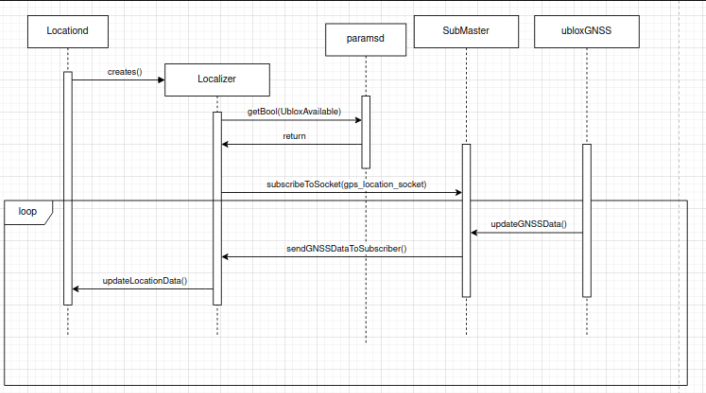
\includegraphics[scale=0.5]{LocationdSequence.png}
    \caption{Sequence diagram for \texttt{locationd}}
    \label{fig:enter-label}
\end{figure}


\begin{figure}[H]
    \centering
    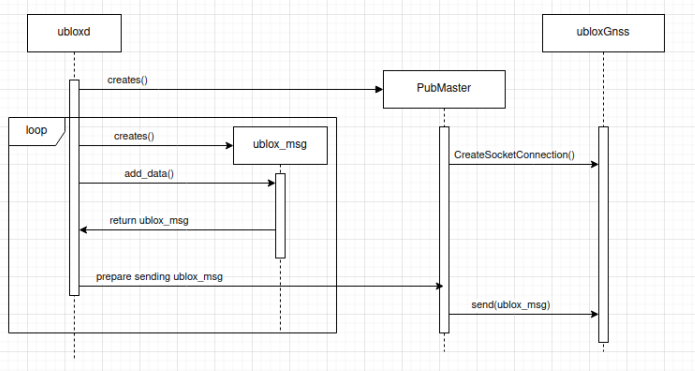
\includegraphics[scale=0.5]{UbloxSequence.png}
    \caption{Sequence diagram for \texttt{ubloxd}}
    \label{fig:enter-label}
\end{figure}

\section{Discussions of The Limitations of Reported Findings}
Our exploration into OpenPilot's architecture provided enlightening insights, albeit with certain limitations that warrant consideration. Our analysis primarily focused on specific components such as \texttt{locationd}, \texttt{calibrationd}, and \texttt{ubloxd}, which allowed for a detailed examination of their inner workings and interactions within the system. However, this targeted approach may have inadvertently overlooked broader system aspects, such as higher-level architectural patterns or cross-cutting concerns like security and error handling.

Additionally, our findings were derived from examining OpenPilot version 0.9.5, a snapshot in time that inherently limits the generalizability of our conclusions. With the platform continuously evolving and new versions, like 0.9.6, already released, there's a possibility that our insights may not fully apply to newer iterations. This underscores the dynamic nature of software development and the need for ongoing analysis and adaptation to keep pace with evolving technologies.

While the use of the Understand tool allowed for a comprehensive exploration of the software's structure, it's important to acknowledge its inherent limitations. While static analysis provides valuable insights into the codebase's organization and dependencies, it inherently lacks the ability to capture the system's dynamic, real-time behaviors. As such, our understanding may be limited to the structural aspects of OpenPilot's architecture, with nuances in system behavior potentially left unexplored.

\section{Data Dictionary}

    \begin{itemize}

        \item[] \textbf{comma three}: The device mounted in the car that the driver interacts with. It has an integrated panda within the system. Comma three runs on a Ubuntu based operating system [5]. It contains three HDR cameras, two to watch the road and one night vision camera to point inside of the car to watch the driver. This assists with the driver attentiveness system [6].
        \item[] \textbf{CAN Bus}: Message based protocol that allows components of the vehicle, called Electric Control Units, to communicate with each other [7].
        \item[] \textbf{Neural Network}: The machine learning model that openpilot uses to predict where the car should go given the input from modeld [5][4].
        \item[] \textbf{GNSS}: Satellites that provide positioning, navigation, and timing services. GPS is an example of a GNSS [8].
        \item[] \textbf{cereal}: Messaging system between robotic systems. Utilizes a publisher and subscriber model [5].
        \item[] \textbf{Understand}: A software tool developed by scitools used for extracting dependencies and architectural diagrams for software projects via source code analysis.
        \item[] \textbf{ubloxGNSS}: The module responsible for receiving and making raw gps data available to other modules 
        \item[] \textbf{ubloxmsg}: message objects created that contain gps data
        \item[] \textbf{PubMaster}: Responsible for managing all the publishers making data published to itself available to other modules
        \item[] \textbf{SubMaster}: Responsible for managing all the subscribers and makes sure that all subscribers recieve the data they are subscribed to. 
        \item[] \textbf{Localizer}: Intermediate module that setup and manages subscription to location data on behalf of Locationd
    \end{itemize}

\section{Naming Conventions}

    \begin{itemize}

        \item[] \textbf{CAN}: Controller Area Network
        \item[] \textbf{DBC}: Database CAN
        \item[] \textbf{GNSS}: Global Navigation Satellite System
        \item[] \textbf{GPS}: Global Positioning System
        \item[] \textbf{IMU}: Inertial Measurement Unit
        \item[] \textbf{UI}: User Interface
        

    \end{itemize}

\section{Lessons Learned}
Through our in-depth analysis, several key lessons emerged that shed light on the intricacies of software architecture and its practical implications, with a specific focus on the architecture design of OpenPilot. We recognized the immense value of analysis tools like Understand, whose capabilities proved invaluable for dissecting the complex interdependencies within OpenPilot's architecture. These tools facilitated a granular examination of subsystem relationships, aiding in our understanding of how different components interact to achieve system functionality. Moreover, our study served as a bridge between theoretical concepts and their real-world application, exemplified by our discussions in Assignment 1. By applying academic knowledge to practical scenarios, we gained a deeper appreciation for the complexities inherent in software development and the critical role of architectural design in shaping system behavior and performance.

Additionally, our analysis underscored the significance of modular architecture in managing the complexity of large-scale software systems. The layered, pipe-and-filter architecture, and modular design principles embraced by OpenPilot enhance our ability to isolate functionalities and understand system behavior, ultimately contributing to system maintainability and scalability. In focusing on the architecture design of OpenPilot, we gained insights into the deliberate decisions and trade-offs made to achieve the system's objectives. The layered and modular approach adopted by OpenPilot reflects a deliberate prioritization of flexibility and scalability, enabling the system to adapt to evolving requirements and technological advancements. By understanding the rationale behind these architectural choices, we can better appreciate the system's strengths and identify areas for improvement.
\section{Conclusion}
In conclusion, our comprehensive study of OpenPilot's architecture has deepened our understanding of autonomous vehicle software and highlighted important considerations for future research and development efforts. We recognize the critical role of clear and well-organized architectural design in the development and maintenance of complex systems like OpenPilot. The layered and modular approach adopted by OpenPilot reflects a deliberate prioritization of flexibility and scalability, enabling the system to adapt to evolving requirements and technological advancements. Looking ahead, we acknowledge the importance of continuous learning and adaptation in software architecture analysis as technology continues to evolve. By embracing a mindset of continuous improvement and innovation, we can ensure that our methodologies remain relevant and effective in addressing the challenges and opportunities presented by emerging technologies in the field of autonomous driving.

\begin{thebibliography}{00}

    \bibitem{b1} “How openpilot works in 2021,” comma.ai, \url{https://blog.comma.ai/openpilot-in-2021/} (accessed Feb. 13, 2024). 

    \bibitem{b2} S. Anumakonda, “The state of comma.ai,” Medium.com, \url{https://srianumakonda.medium.com/the-state-of-comma-ai-2140aabc6f52} (accessed Feb. 13, 2024).

    \bibitem{b3} “openpilot 0.9.5,” comma.ai, \url{https://blog.comma.ai/095release/} (accessed Feb. 13, 2024).

    \bibitem{b4} “Openpilot - Open source advanced driver assistance system,” comma.ai, \url{https://comma.ai/openpilot} (accessed Feb. 13, 2024).

    \bibitem{b5} “From vision to architecture: How to use openpilot and live,” From Vision To Architecture: How to use openpilot and live - DESOSA 2020, \url{https://desosa.nl/projects/openpilot/2020/03/11/from-vision-to-architecture} (accessed Feb. 13, 2024).

    \bibitem{b6} “Comma 3x - make driving chill,” comma.ai, \url{https://comma.ai/shop/comma-3x} (accessed Feb. 13, 2024). 

    \bibitem{b7} G. M. Smith, “What Is CAN Bus (Controller Area Network) and How It Compares to Other Vehicle Bus Networks,” dewesoft.com,
    \url{https://dewesoft.com/blog/what-is-can-bus} (accessed Feb. 14, 2024).
    
    \bibitem{b8} “Other Global Navigation Satellite Systems (GNSS),” Gps.gov, Oct. 19, 2021.
    \url{https://www.gps.gov/systems/gnss/#:~:text=Global%20navigation%20satellite%20system%20(GNSS,a%20global%20or%20regional%20basis} (accessed Feb. 14, 2024).

\end{thebibliography}
\end{document}